%
% HR.tex
% Human Resources
%
% Aleph Objects Operations Manual
%
% Copyright (C) 2014, 2015 Aleph Objects, Inc.
%
% This document is licensed under the Creative Commons Attribution 4.0
% International Public License (CC BY-SA 4.0) by Aleph Objects, Inc.
%

%
% HR.tex
% Human Resources
%
% Aleph Objects Operations Manual
%
% Copyright (C) 2014, 2015 Aleph Objects, Inc.
%
% This document is licensed under the Creative Commons Attribution 4.0
% International Public License (CC BY-SA 4.0) by Aleph Objects, Inc.
%

\section{Job Descriptions}
Aleph Objects job descriptions. Needs cleanup, many descriptions are job ads or requests.

\subsection{3D Printer Technician}
Job responsibilities include running a cluster of 144 3D printers, repairing and maintaining printers, part production planning, and part processing and inspection.

Experience with 3D printers is highly desired but not required. General knowledge of mechanical equipment is a plus. Basic computer skills are required and experience with GNU/Linux is a plus. Time management is a MAJOR factor of this position including managing part production quotas, timelines, and deadlines.

The LulzBot fleet runs 24 hours a day; day, evening, or night shifts are a possibility. This position requires standing the majority of the work day. On occasion this position requires lifting 30-40 lb packages.

\subsection{Assembler}
Major job duties include:

\begin{itemize}
 \item Assemble fabricated parts at floor stations.
 \item Use hand tools and power tools to assemble units according to product specifications.
 \item Test and calibrate parts and mechanisms to meet tolerances and product specifications.
 \item Identify units that fail tests or tolerance levels and repair as necessary.
 \item Rely on instructions and pre-established guidelines to perform the functions of the job.
 \item Flexible and can perform a variety of tasks.
\end{itemize}

This position requires a high school diploma or its equivalent. May be required to complete an apprenticeship and/or formal training in area of specialty. Prefers 2-5 years of industry experience.

\subsection{Copywriter}
Supervisor: Marketing Manager

Description: Your job is to use written words to facilitate the development, sale, use, and support of LulzBot products. You will work cross-functionally with other departments to ensure the company is effectively using words to communicate with internal and external stakeholders.

Role and Responsibilities:
\begin{itemize}
 \item Work with Research and Development to establish and enhance internal documentation for prospective, current, and past products.
 \item Work with Customer Support to improve support documentation and service bulletins for internal and external use, including the Forum and Wiki as-needed.
 \item Work with Creative to develop and improve packaging, documentation, instructions, web design, promotional materials, advertisements, and more.
 \item Work with Marketing to write copy for social media, newsletter, product pages, interviews, press releases, and more, as well as attend events and trade shows.
 \item Work with Sales to develop sales collateral, including templates and call scripts.
 \item Work with other departments as-needed to ensure the company's use of written language reflects the brand across all platforms, at all times.
 \item Utilize strong verbal skills for presentations to internal and external stakeholders.
 \item Edit and proofread copy for accuracy, grammar and punctuation, including reviewing final copy for preproduction used on the website, in video, and other deliverables.
 \item Utilize an organized, comprehensible method for storing revisions and documents for easy use and collaboration with others.
 \item Help with other tasks as-needed to grow the company, serve its customers, and advance Free Software, Libre Innovation, and Open Source Hardware (FLO).
\end{itemize}

Work Experience:
3+ years as a Copywriter, Editor, Proofreader, or Technical Documentation Writer.
Environments requiring creating a high volume of quality content at a fast pace. 
Professional use of desktop 3D printing is preferred, especially Free Software, Libre Innovation, and Open Source Hardware (FLO) tools and Free Culture licenses.

Skills, Certifications, and Education:
\begin{itemize}
 \item Bachelor’s degree in Marketing, Communications, Creative Writing, or Liberal Arts is preferred.
 \item Excellent typist with an ability to type a high number of words per minute with accuracy.
 \item A meticulous writer with an eye for editing and proofing.
 \item Exceptional ability to manage multiple projects simultaneously, set priorities, pro-actively identify and address problems, and meet deadlines.
 \item Proficiency in productivity tools including word processing and spreadsheets.
 \item Experience with HTML, CSS, and creative applications (e.g. Scribus, Inkscape, \LaTeX) a plus.
\end{itemize}

Travel Expectations
Approximately 10-20\%, including possible international travel.

\subsection{Creative Manager}
Supervisor: Chief Operating Officer

Description: Your primary responsibilities will be to oversee the overall creative design of the company’s marketing materials, products, packaging, and documentation. Your role as Creative Manager will be cross-functional, engaging with other departments throughout the company as well as vendors and customers to ensure that the look and feel of company output is consistent with achieving the company's strategic goals.

Role and Responsibilities:
\begin{itemize}
 \item Work collaboratively with the Marketing to plan and develop new and exciting creative assets that uphold the strategic goals of the brand.
 \item Provide creative support company-wide including the design or design direction of logos, icons, and other digital assets, advertisements, trade-show visuals, email campaigns, social media pages, software UI, product packaging, 3D printed object designs, investor relations materials, and print collateral.
 \item Collaborate with Research and Development, contributing to UI development, product industrial design, and ensuring overall output is aligned with company creative and branding strategy. 
 \item Work with Purchasing to manage vendor communications pertaining to creative and brand strategy.
 \item Capture, organize, and prepare photo and video assets for use in marketing and product documentation.
 \item Study the marketplace, continually assessing where the company stands in relation to its competition from a creative and branding perspective.
 \item Research, vet, and communicate with outside creative resources including printers, photographers, videographers, and freelancers.
 \item Supervise and schedule creative personnel including graphic designers, photographers, videographers, and 3D artists.
 \item Quality control, including proofing and reviewing of creative output.
 \item Organize digital and analog department documents for easy use and collaboration with others.
\end{itemize}

Work Experience:
\begin{itemize}
 \item 3 Years of related experience
 \item Superior understanding of visual composition and advertising principles
 \item Superior knowledge and practical application across a wide range of creative software tools (experience with Free Software such as GIMP, Inkscape, Kdenlive, and Scribus is a helpful) 
 \item Demonstrated competence with photo/video hardware and lighting
 \item 3D modeling, animation, and 3D printing experience is preferred
 \item HTML, CSS, and any other back-end web development experience a plus
 \item A strong portfolio of both digital and print design available for review
\end{itemize}

Travel Expectations
No more than 10\%, including possible international travel.

\subsection{Customer Support Representative}
Job responsibilities include answering support phone calls and emails. Other tasks may be delegated as needed, depending on experience. Experience with 3D printers, specifically LulzBot and RepRap hardware printers and hardware, is highly desired. Support inquiries will range from LulzBot.com store functions, such as customer account and shipping questions, to technical questions about LulzBot 3D printers and hardware.

\subsection{Manufacturing Engineering}
Role: Representing MFG, act as a single contact point working with R\&D to provide and implement solution and/or corrective actions on all engineering and process related issues.

Job Scope:
\begin{itemize}
 \item Get trained, understand, and implement new design or design changes generated by R\&D into manufacturing
 \item Provide feedback and suggestions regarding engineering designs to R\&D to improve reliability or to enhance the manufacturability of the product.
 \item Actively work with R\&D to resolve design-related, process-related (as recommended by R\&D), or material related issues that might have an impact on product quality/reliability or production output including performing failure analysis and design of experiment when need be.
 \item Design and implement new processes in manufacturing to improve product quality/reliability, production output. Consult with R\&D when appropriate especially if the change might impact the performance and/or functionality of the product.
 \item Be an active member and take part in the new product launch process. Provide manufacturing engineering readiness plan with actions and targets to timely support the new product launch.
 \item Install/implement, maintain and provide training on all manufacturing equipments. Initiate requests to R\&D and collaborate with R\&D on design and implement of custom in-house built tools and test test equipment.
\end{itemize}

\subsection{Manufacturing Technician I}
Operates production equipment; responsible for manufacturing and assembly of clinical and commercial products. Follows blueprints, guidelines and/or diagrams to ensure product specifications and tolerance levels are met. Requires a high school diploma or its equivalent and 0-3 years of related experience. Has knowledge of commonly-used concepts, practices, and procedures within a
particular field. Relies on instructions and pre-established guidelines to perform the functions of the job. Works under immediate supervision. Typically reports to a supervisor.

\subsection{Manufacturing Technician II}
Operates production equipment; responsible for manufacturing and assembly of clinical and commercial products. Follows blueprints, guidelines and/or diagrams to ensure product specifications and tolerance levels are met. Requires a high school diploma or its equivalent and 2-5 years of related experience. Familiar with standard concepts, practices, and procedures within a particular field. Relies on limited experience and judgment to plan and accomplish goals. Performs a variety of tasks. Works under general supervision. A certain degree of creativity and latitude is required. Typically reports to a supervisor.

\subsection{Manufacturing Technician III}
Operates production equipment; responsible for manufacturing and assembly of clinical and commercial products. Follows blueprints, guidelines and/or diagrams to ensure product specifications and tolerance levels are met. Requires a high school diploma or its equivalent and at least 5 years of related experience. Familiar with a variety of the field's concepts, practices, and procedures. Relies on
extensive experience and judgment to plan and accomplish goals. Performs a variety of tasks. May lead and direct the work of others. A wide degree of creativity and latitude is expected. Typically reports to a supervisor or manager.

\subsection{Marketing Associate}
Supervisor: Marketing Manager

Description: Your job is to engage current and prospective customers through interactive experiences, including events, social media, and email, to grow the LulzBot community. You will be working primarily within the marketing department to help increase brand awareness and sales.

Role and Responsibilities:
\begin{itemize}
 \item Work with Marketing to evaluate, propose, and execute the company's attendance at events.
 \item Work with Marketing to maintain the company's social media accounts, and specifically be able to evaluate, propose, and execute digital advertising campaigns.
 \item Work with Marketing to conduct customer surveys and other forms of market research.
 \item Work with Marketing to incorporate feedback from events, social media, and the newsletter into research and development, new product introduction, purchasing, sales, and other departments' activities as-needed.
 \item Work with Creative to facilitate in the creation of packaging, documentation, instructions, web design, promotional materials, advertisements, and more as-needed.
 \item Work with Sales to facilitate the staffing, training, and attendance of events.
 \item Utilize strong verbal skills for presentations to internal and external stakeholders.
 \item Edit and proofread copy for accuracy, grammar and punctuation.
 \item Utilize an organized, comprehensible method for storing revisions and documents for easy use and collaboration with others.
 \item Help with other tasks as-needed to grow the company, serve its customers, and advance Free Software, Libre Innovation, and Open Source Hardware (FLO).
\end{itemize}

Work Experience:
Minimum of 1 – 3 years relevant experience
Environments requiring complex coordination of logistical activities that are subject to change.
Sophisticated understanding of the risks and opportunities associated with large-scale communication (including email newsletters, social media, etc.) 
Professional use of desktop 3D printing is preferred, especially Free Software, Libre Innovation, and Open Source Hardware (FLO) tools and Free Culture licenses.

Skills, Certifications, and Education:
Bachelor’s degree in Marketing, Communications, or Liberal Arts is preferred.
A meticulous writer with an eye for editing and proofing, and inclusive communicator (with regard to race, color, religion, gender, gender identity or expression, sexual orientation, national origin, genetics, disability, age, and veteran status).
Exceptional ability to manage multiple projects simultaneously, set priorities, pro-actively identify and address problems, and meet deadlines.
Proficiency in mass communication tools (e.g. phpList, LimeSurvey) and social media.

Travel Expectations
Approximately 10-20\%, including possible international travel.

\subsection{Marketing Manager}
Supervisor: Chief Operating Officer

Description: Your job is to establish, develop, promote and protect the brand of LulzBot products through marketing activities. You will be working cross-functionally with other department leaders in various capacities to coordinate strategic decision-making, activities, schedules, budgets, partnerships, and products to help grow the company and increase sales.

Role and Responsibilities:
\begin{itemize}
 \item Work with Research and Development to manage feasibility and testing of new products, including (but not limited to) 3D printers, accessories, and materials.
 \item Work with Customer Support to manage documentation, service bulletins, Forum and Wiki updates as-needed to ensure consistent customer experience.
 \item Work with Creative (within Marketing) to manage strategy and execution of packaging, documentation, instructions, web design, promotional materials, advertisements, and more.
 \item Work with Marketing to manage social media, newsletter, product pages, interviews, public relations, government affairs, outside vendors, analytics, events and trade shows, and more.
 \item Work with Shipping to manage the delivery and return of materials as-needed.
 \item Work with Purchasing to manage vendor communications and relationships as-needed.
 \item Work with Finance and Accounting to develop budgets, investor relations materials, assist with sales projections and market strategy as-needed.
 \item Work with Sales to manage communication with Marketing and development of sales collateral, including templates and call scripts, sales projections, and more.
 \item Ensure consistent use of the company's brand across all platforms, at all times.
 \item Utilize strong verbal skills for presentations to internal and external stakeholders.
 \item Utilize an organized, comprehensible method for department documents for easy use and collaboration with others.
 \item Help with other tasks as-needed to grow the company, serve its customers, and advance Free Software, Libre Innovation, and Open Source Hardware (FLO).
\end{itemize}

Work Experience:
3+ years relevant experience in sales and/or marketing in rapidly changing environments.
Experience applying varied marketing and new product introduction strategies.
Experience leading teams in a fast pace environment to achieve excellent outcomes.
Deep knowledge of—or, aptitude for quick learning about—the 3D printing industry, and Free Software, Libre Innovation, and Open Source Hardware (FLO) tools and Free Culture licenses.

Skills, Certifications, and Education
Bachelor’s degree in Business, Marketing, Communications, or Liberal Arts is preferred.
Exceptional ability using quantitative data and qualitative insights for strategic decision-making.
Pro-active communicator comfortable with directly reporting to executive leadership.

Travel Expectations
Approximately 10-20\%, including possible international travel.

\subsection{Office Manager}
Facility:
Works with the facilities manager and outside contractors to respond to routine maintenance needs.  
Offers feedback to executives for proposed facility changes and future needs.
Keep a sign up schedule for the conference room.

Office Supply:
Periodically review office supply inventory.  
Field employee office supply requests.  
Create consolidated weekly purchase requests for office supplies.
Purchase urgently needed supplies.

Human Resources:
\begin{itemize}
 \item Reply to all submissions to jobs@alephobjects.com, forward submissions to PEO or hiring managers for open positions.
 \item Work with Managers and Insperity recruiting and on-boarding new employees.
 \item Process employee background screening requests.
 \item Maintain confidential employee files.
 \item Answer questions from employees with Human Resource needs.
 \item Ensure compliance with local, state, and federal laws related to Human Resource needs.
 \item Assist Managers with employee coaching and discipline, and termination procedures.
 \item Work with Insperity to offer performance and liability training.
 \item Work with manager and Insperity to create and implement company policies.
 \item Assist Managers with establishing periodic performance reviews process.
\end{itemize}

Other:
\begin{itemize}
 \item Assist Executives with corporate record keeping.
 \item Assist Executives with corporate licensing administration.
 \item Assist with hospitality events.
\end{itemize}

Requirements:
\begin{itemize}
 \item office administration experience
 \item verbal and written communication skills
 \item office software skills
 \item attention to detail
 \item ability to work cross-functionally within the enterprise
\end{itemize}

\subsection{Purchasing Assistant}
In this role you have the daily responsibility in maintaining procurement activities required to meet the needs of current projects utilizing existing Bill of Materials (BOM). Additionally, you will be monitoring supplier activity to ensure optimal performance and quality for all purchases.
 
Key Responsibilities: 

\begin{itemize}
 \item Maintain and update Inventory \& Bill of Material database
 \item Become familiar with materials and manufacturing processes
 \item Assist in determining purchasing needs through inventory maintenance activities
 \item Maintain procurement records such as items or services purchased; costs; delivery; product quality or performance, and inventories.
 \item Prepare quote requests and purchase orders
 \item Communicates with vendors on lead time and logistics for orders
 \item Organizing and tracking purchase order confirmations
\end{itemize}

Requirements:

High School Diploma or equivalent; Associate or Bachelor Degree in related field a plus
Minimum of 2 years prior experience in a Purchasing capacity, preferably in a manufacturing enterprise
Proficient with office software and word processing applications, strong spreadsheet skills 
Previous experience with ERP or MRP systems is preferred
Excellent oral and written communication skills
Detail oriented and well organized
High level of initiative and independent judgment

\subsection{Receptionist}
Job duties include greeting customers, answering and screening phone calls and emails, sorting and distributing mail, taking lunch orders, raising and lowering the Aleph Objects flags, and performing basic administrative support tasks. Other duties may be delegated, depending on experience.

Basic computer skills are required. Any experience with the GNU/Linux operating system is welcomed.

\subsection{Sales Account Manager}
Essential Functions:
\begin{itemize}
 \item Oversee and manage existing account relationships
 \item Develop and manage new account relationships through incoming leads and lead generation strategies.
 \item Coordinating with others within the company to insure high levels of customer satisfaction
 \item Periodically attend events and trade shows to develop new accounts
 \item Work with management to maintain and approve processes
\end{itemize}

Desired skills include:
\begin{itemize}
 \item Must be customer focused and service oriented
 \item Ability to develop a complete and broad technical knowledge of products and industry trends
 \item Ability to learn new skills, adapt to changing environments and show attention to detail
 \item Good organizational skills
 \item Strong interpersonal skills and an ability to work with teams
 \item Excellent communication (both written and verbal) and presentation skills
 \item Proficient problem solving and analytical ability
 \item Must be proficient with office productivity software
\end{itemize}

EDUCATION/EXPERIENCE REQUIREMENTS
High School Diploma or equivalent is required
Associates Degree in related field preferred
2-3 years sales experience preferred

\subsection{Sales Manager}
Essential Functions:
\begin{itemize}
 \item Oversee and manage existing account relationships
 \item Develop and manage new account relationships through incoming leads and lead generation strategies.
 \item Coordinating with others within the company to insure high levels of customer satisfaction
 \item Periodically attend events and trade shows to develop new accounts
 \item Work with management to maintain and approve processes
\end{itemize}

Desired skills include:
\begin{itemize}
 \item Must be customer focused and service oriented
 \item Ability to develop a complete and broad technical knowledge of products and industry trends
 \item Ability to learn new skills, adapt to changing environments and show attention to detail
 \item Good organizational skills
 \item Strong interpersonal skills and an ability to work with teams
 \item Excellent communication (both written and verbal) and presentation skills
 \item Proficient problem solving and analytical ability
 \item Must be proficient with office productivity software
\end{itemize}

EDUCATION/EXPERIENCE REQUIREMENTS
High School Diploma or equivalent is required
Associates Degree in related field preferred
2-3 years sales experience preferred

\subsection{Sales Support Associate}
ESSENTIAL FUNCTIONS:
Responsible for verifying that all files, computer generated shared documents, sales quotations, and sales orders, are current, accurate, and accessible.

Verify and process internet sales orders

Receives incoming calls, assist customers on the phone with inside sales orders

Respond to customer sales leads via email responding to incoming correspondence and ensure a timely response.

Handles a variety of sensitive situations advising the sales manager of actions taken.  Independently responds to customer calls and emails.

Act as final review of all completed sales orders prior to shipment.

Provides feedback for streamlining processes and increasing efficiency for the sales department.

Maintains a professional office environment at all times.

EDUCATION/EXPERIENCE REQUIREMENTS
High School Diploma or equivalent is required.  Associates Degree in related field preferred
Three to five years progressively responsible clerical experience preferably sales office experience.
Attention to detail
typing speed > 40 wpm

\subsection{Sales Support Specialist}
ESSENTIAL FUNCTIONS:
Responsible for verifying that all files, computer generated shared documents, sales quotations, and sales orders, are current, accurate, and accessible.

Verify and process internet sales orders

Receives incoming calls, assist customers on the phone with inside sales orders

Respond to customer sales leads via email responding to incoming correspondence and ensure a timely response.

Handles a variety of sensitive situations advising the sales manager of actions taken.  Independently responds to customer calls and emails.

Assigned special tasks by management including one off tasks, testing and assisting and developing new processes, and providing feedback to management on existing processes.

Act as final review of all completed sales orders prior to shipment.

Provides feedback for streamlining processes and increasing efficiency for the sales department.

Maintains a professional office environment at all times.

EDUCATION/EXPERIENCE REQUIREMENTS
High School Diploma or equivalent is required.  Associates Degree in related field preferred
Three to five years progressively responsible clerical experience preferably sales office experience.
Attention to detail
typing speed > 40 wpm

\subsection{Senior Accountant}
\begin{itemize}
 \item Preparing and/or reviewing all aspects of financial accounting, from journal entries through month-end close.
 \item Prepare analysis, schedules and calculations which support month-end financial reporting.
 \item Collaborations with the manufacturing and sales team on various projects.
 \item Ensure compliance with taxation across multiple jurisdictions.
 \item Work with manufacturing and operations to expand understanding and application of OpenERP system as well as improving Company information systems with appropriate level of controls.
 \item Act as liaison with third party PEO organization, including updating and reporting of payroll transactions.
 \item Be willing to work on various projects independently.
 \item Ad hoc analysis.
 \item Supervision of bookkeeper.
\end{itemize}

\subsection{Technical Support Representative}
ESSENTIAL FUNCTIONS:
Responsible for verifying that all files, computer generated shared documents, sales quotations, and sales orders, are current, accurate, and accessible.

Verify and process internet sales orders

Receives incoming calls, assist customers on the phone with inside sales orders

Respond to customer sales leads via email responding to incoming correspondence and ensure a timely response.

Handles a variety of sensitive situations advising the sales manager of actions taken. Independently responds to customer calls and emails.

Act as final review of all completed sales orders prior to shipment.

Provides feedback for streamlining processes and increasing efficiency for the sales department.

Maintains a professional office environment at all times.

EDUCATION/EXPERIENCE REQUIREMENTS
Three to five years progressively responsible clerical experience preferably sales office experience.
Attention to detail
typing speed > 40 wpm

\subsection{Webmaster}
The webmaster is responsible for keeping the e-Commerce website up to date.

Responsibilities:
Maintain the e-Commerce website by adding features as needed using GNU/Linux with Apache web server
Admin website using Python, PHP, SQL and the data programming language
 
Qualifications:
\begin{itemize}
 \item Experience with ERP system, Piwik, Drupal Commerce, Ubercart
 \item GNU/Linux experience a must
 \item Experience with Python and Django a plus
 \item Project management experience
 \item Must be self-reliant
\end{itemize}
 


\section{Professional Employment Organizations (PEO)}
Insperity.

\section{Employee Benefits}
See employee handbook at \texttt{http://esc.insperitiy.com}

\section{Logging hours in OpenERP}
For hourly Insperity employees:

OpenERP ---> Human Resources ---> Attendences ---> Attendences

For hourly Kelly employees, track your hours on Kelly's website.

\section{Requesting time off in OpenERP}
OpenERP ---> Human Resources ---> Leaves ---> Leave Requests

\section{Recruitment / Interviewing}
Kelly, Insperity, JobZology.

\section{Performance}
Insperity.

\section{Training}
Certifications.

\section{Organizational Chart}
See figure \ref{fig:ao_org_chart} for Aleph Object's organizational chart.
%
% OrgChart.tex
% HR Organizational Chart
%
% Aleph Objects Operations Manual
%
% Copyright (C) 2014, 2015 Aleph Objects, Inc.
%
% This document is licensed under the Creative Commons Attribution 4.0
% International Public License (CC BY-SA 4.0) by Aleph Objects, Inc.

\begin{sidewaysfigure}[p]
\thisfloatpagestyle{empty}
\begin{center}
\resizebox{\textwidth}{!}
{
\begin{forest}
for tree={
  draw,
  minimum height=3cm,
  anchor=north,
  align=center,
  child anchor=north,
  inner sep=5mm,
  s sep=5mm
},
[{CEO}, align=center, for tree={rectangle}, fill=ao-purple, tier=first
    [{CTO}, for tree={fill=pink}, tier=second, child anchor=east
        [{Engineer\\Assistant}, tier=third
            [{Cluster\\Tech}, tier=fourth]
            [{Cluster\\Tech}, tier=fourth]
        ]
        [{Engineer\\Assistant}, tier=third]
      [{VP Mfg}, for tree={fill=ao-light-orange}, tier=third
            [{Assembly\\Lead}, for tree={fill=ao-light-orange}, tier=fourth
                [{Assembly\\I}, tier=fifth]
                [{Assembly\\I}, tier=fifth]
                [{Assembly\\II}, tier=fifth]
                [{Assembly\\II}, tier=fifth]
                [{Assembly\\II}, tier=fifth]
                [{Assembly\\II}, tier=fifth]
            ]
        ]
    ]
    [{Bookkeeper}, fill=ao-gold], tier=second
    [{SysAdmin}, fill=ao-dark-blue], tier=second
    [{COO}, for tree={fill=ao-light-blue}, tier=second child anchor=west
        [{Shipping\\Manager}, tier=third]
        [{Sales\\Manager}, tier=third]
        [{Programmer}, tier=third]
        [{Comms}, tier=third]
        [{CSR}, tier=third]
    ]
]
\end{forest}
}
\end{center}
\caption{Organizational Chart}
 \label{fig:ao_org_chart}
\end{sidewaysfigure}


See figure \ref{fig:ao_org_chart_dot} for Aleph Object's organizational chart in dot.

\begin{sidewaysfigure}[p]
\thisfloatpagestyle{empty}
% The ao-orgchart-dot.png was built in dot.
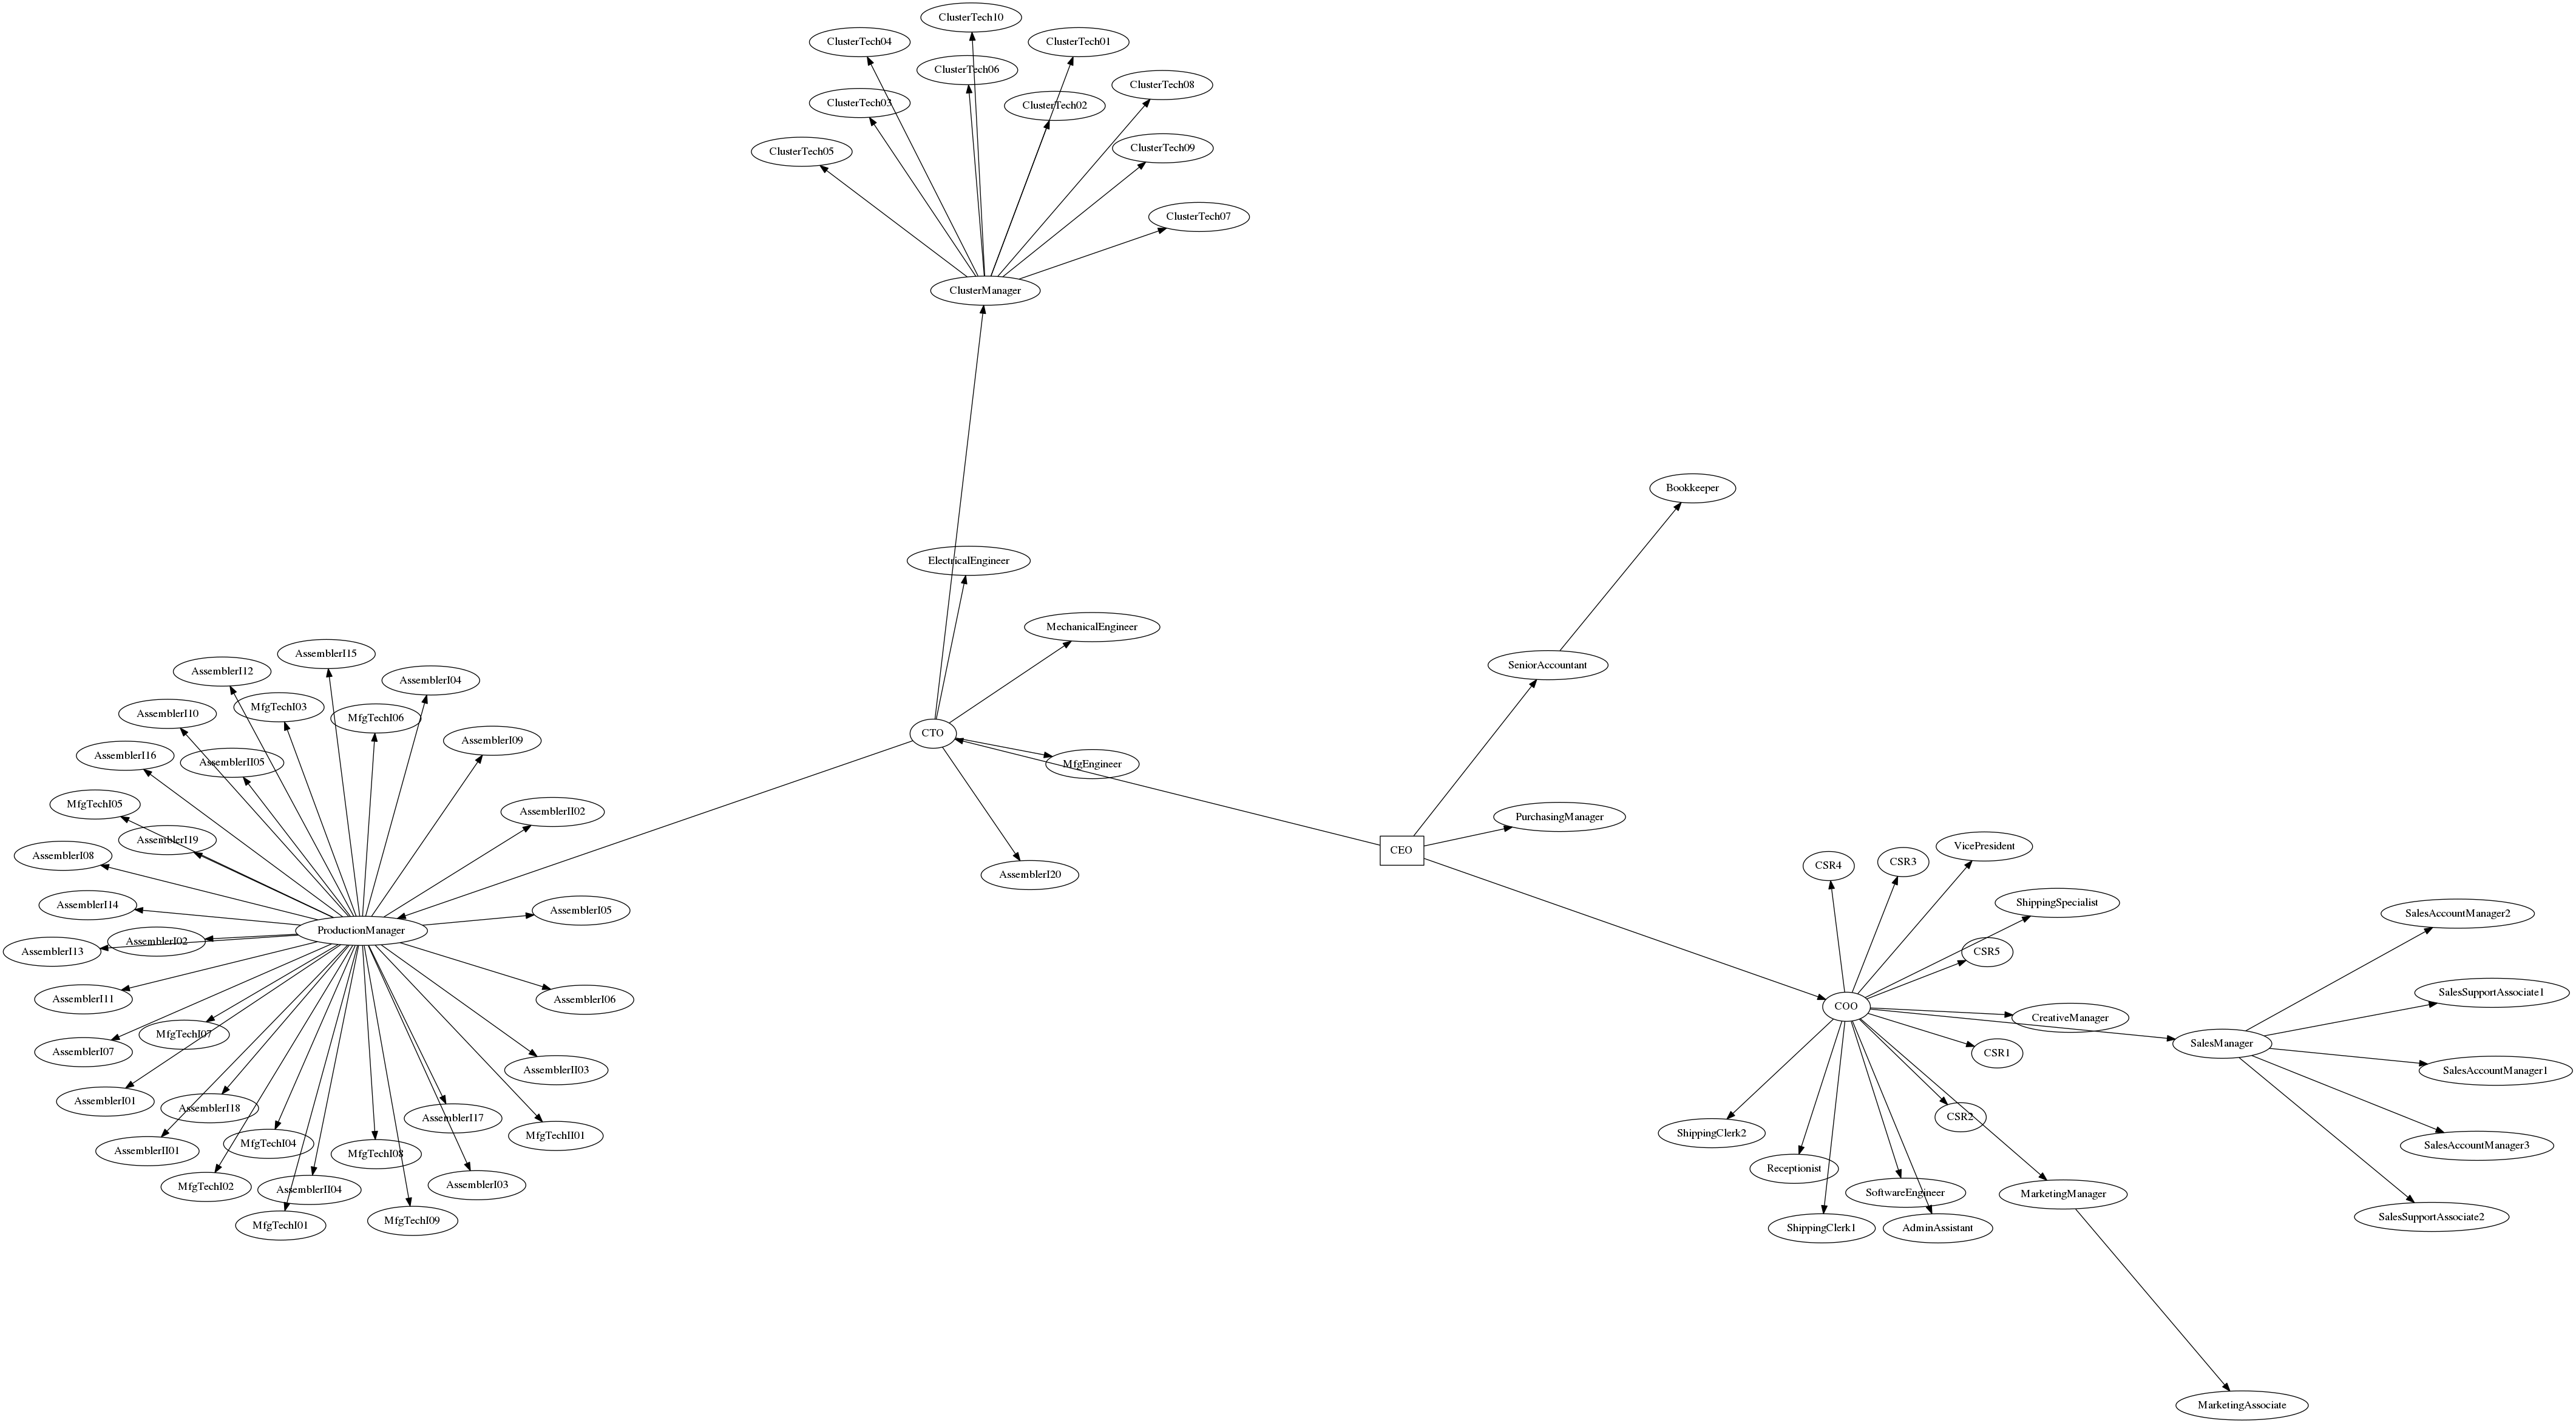
\includegraphics[keepaspectratio=true,height=1.10\textheight,width=1.00\textwidth,angle=-90]{ao-orgchart-dot.png}
 \caption{Aleph Objects Org Chart dot}
 \label{fig:ao_org_chart_dot}
\end{sidewaysfigure}

\section{Schedules}
The following calendars list when there are recurring meetings.

%
% SchedWeek.tex
% Weekly Recurring Events Schedule
%
% Aleph Objects Operations Manual
%
% Copyright (C) 2014 Aleph Objects, Inc.
%
% This document is licensed under the Creative Commons Attribution 4.0
% International Public License (CC BY-SA 4.0) by Aleph Objects, Inc.
%

% To extract just the schedule pages from the PDF, run something like:
% pdfjoin AOOM.pdf 31-32 -o AOOM-schedule.pdf

% These set the width of a day and the height of an hour.
\newcommand*\daywidth{3.7cm}
\newcommand*\hourheight{3.8em}

% The entry style will have two options:
% * the first option sets how many hours the entry will be (i.e. its height);
% * the second option sets how many overlapping entries there are (thus
%   determining the width).
\tikzset{entry/.style 2 args={
    xshift=(0.5334em+0.8pt)/2,
    draw,
    line width=0.8pt,
    font=\sffamily,
    rectangle,
    rounded corners,
    fill=blue!20,
    anchor=north west,
    inner sep=0.3333em,
    text width={\daywidth/#2-1.2em-1.6pt},
    minimum height=#1*\hourheight,
    align=center
}}

% Start the picture and set the x coordinate to correspond to days and the y
% coordinate to correspond to hours (y should point downwards).
\begin{sidewaysfigure}[p]
\thisfloatpagestyle{empty}
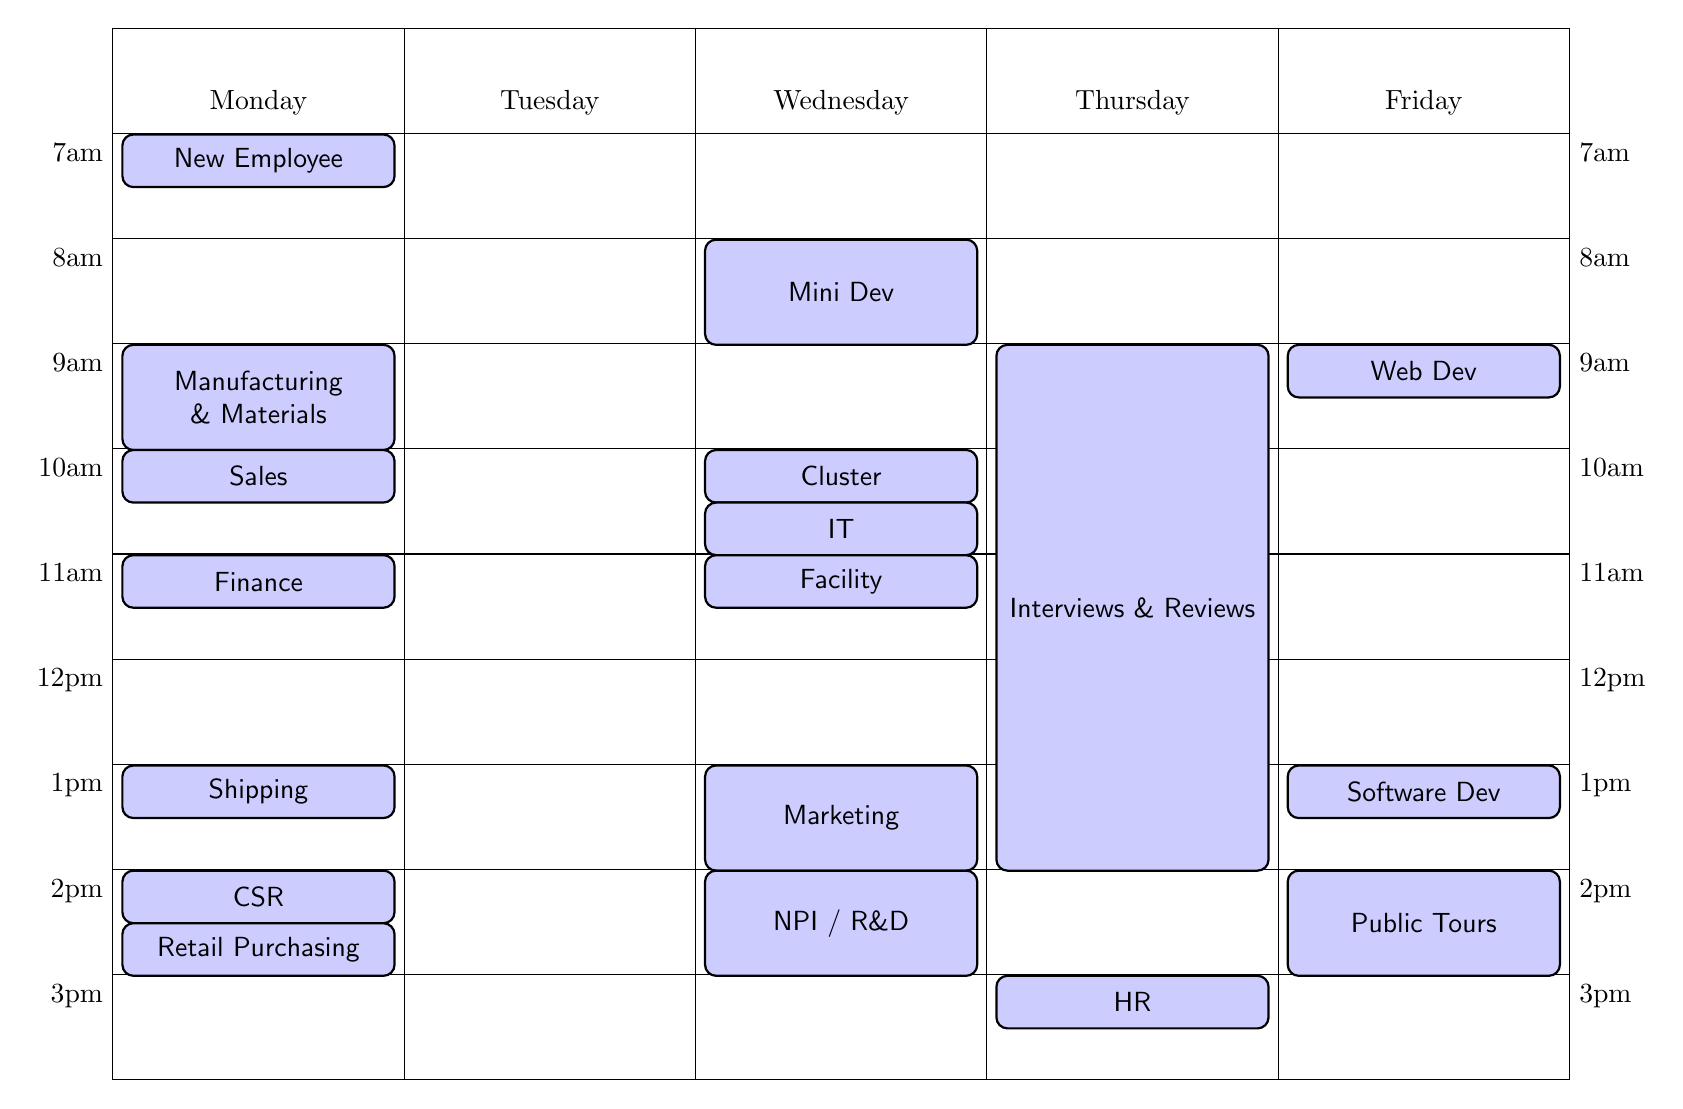
\begin{tikzpicture}[y=-\hourheight,x=\daywidth]

    % First print a list of times.
    \foreach \time/\ustime in {7/7am,8/8am,9/9am,10/10am,11/11am,12/12pm,13/1pm,14/2pm,15/3pm}
        \node[anchor=north east] at (1,\time) {\ustime};

    % Draw some day dividers.
    \draw (1,6) -- (1,16);
    \draw (2,6) -- (2,16);
    \draw (3,6) -- (3,16);
    \draw (4,6) -- (4,16);
    \draw (5,6) -- (5,16);
    \draw (6,6) -- (6,16);
    
    % Draw some hour dividers.
    \draw (1,6) -- (6,6);
    \draw (1,7) -- (6,7);
    \draw (1,8) -- (6,8);
    \draw (1,9) -- (6,9);
    \draw (1,10) -- (6,10);
    \draw (1,11) -- (6,11);
    \draw (1,12) -- (6,12);
    \draw (1,13) -- (6,13);
    \draw (1,14) -- (6,14);
    \draw (1,15) -- (6,15);
    \draw (1,16) -- (6,16);

    \foreach \time/\ustime in {7/7am,8/8am,9/9am,10/10am,11/11am,12/12pm,13/1pm,14/2pm,15/3pm}
        \node[anchor=north west] at (6,\time) {\ustime};
        
    % Start Monday.
    % Write the entries. Note that the x coordinate is 1 (for Monday) plus an
    % appropriate amount of shifting. The y coordinate is simply the starting
    % time.
    % 1=Monday, 2=Tuesday, 3=Wednesday, 4=Thursday, 5=Friday
    %\node[entry={DURATION}{COLUMN WIDTH?}] at (DAY,HOUR) {TEXT};
    \node[anchor=north] at (1.5,6.5) {Monday};
    \node[entry={0.5}{1}] at (1,7) {New Employee};
    \node[entry={1.0}{1}] at (1,9) {Manufacturing \& Materials};
    \node[entry={0.5}{1}] at (1,10){Sales};
    \node[entry={0.5}{1}] at (1,11) {Finance};
    \node[entry={0.5}{1}] at (1,13) {Shipping};
    \node[entry={0.5}{1}] at (1,14) {CSR};
    \node[entry={0.5}{1}] at (1,14.5) {Retail Purchasing};

    % Tuesday
    \node[anchor=north] at (2.5,6.5) {Tuesday};
    
    % Wednesday
    \node[anchor=north] at (3.5,6.5) {Wednesday};
    \node[entry={1.0}{1}] at (3,8) {Mini Dev};
    \node[entry={0.5}{1}] at (3,10) {Cluster};
    \node[entry={0.5}{1}] at (3,10.5) {IT};
    \node[entry={0.5}{1}] at (3,11) {Facility};
    \node[entry={1.0}{1}] at (3,13) {Marketing};
    \node[entry={1.0}{1}] at (3,14) {NPI / R\&D};
    
    % Thursday
    \node[anchor=north] at (4.5,6.5) {Thursday};
    \node[entry={5.0}{1}] at (4,9) {Interviews \& Reviews};
    \node[entry={0.5}{1}] at (4,15) {HR};
    
    % Friday
    \node[anchor=north] at (5.5,6.5) {Friday};
    \node[entry={0.5}{1}] at (5,9) {Web Dev};
    \node[entry={0.5}{1}] at (5,13) {Software Dev};
    \node[entry={1.0}{1}] at (5,14) {Public Tours};

\end{tikzpicture}
\caption{Weekly Company Meetings}
 \label{fig:ao_week_meet}
\end{sidewaysfigure}


See figure \ref{fig:ao_week_meet} for Aleph Object's weekly meeting schedule.
%
% SchedMonth.tex
% Recurring Events Schedule
%
% Aleph Objects Operations Manual
%
% Copyright (C) 2014, 2015 Aleph Objects, Inc.
%
% This document is licensed under the Creative Commons Attribution 4.0
% International Public License (CC BY-SA 4.0) by Aleph Objects, Inc.
%

%%% Monthly Meeting
\newcommand{\calrow}[1]{%
%\node[anchor=base,xshift=0.5ex](sun){S};
%\node[base right=of sun](mon){M};
\node[anchor=base,xshift=0.5ex](mon){M};
\node[base right=of mon](tue){T};
\node[base right=of tue](wed){W};
\node[base right=of wed](thu){T};
%\node[base right=of thu](fri){\ \!F};
%\node[base right=of fri](sat){\ \!S};
\node[base right=of thu](fri){F};
\node[base right=of fri](sat){S};
\node[base right=of sat](sun){S};
\node[black,above=of thu]{\textbf{#1}};
}

\newcommand{\calperiod}[1]{\calendar[dates=\the\year-#1-01 to \the\year-#1-last,
  every day/.style={anchor=base}, % Center days
  day text={\%d=},rounded corners=0,anchor=base,text height=1ex,text depth=-0.5ex]
\holidays;}

% Company Holidays 2015:
% New Year's Day 2015-01-01 - Thursday
% Memorial Day 2015-05-25 - Monday
% Independence Day 2015-07-04 - Saturday
% Labor Day - 2015-09-07 - Monday
% Thanksgiving Day - 2015-11-26 - Thursday
% Day after Thanksgiving - 2015-11-27 - Friday
% Christmas - 2015-12-25 - Friday

% Company meetings, the first business day of the month at 8AM, for 2015.
\newcommand{\holidays}{
if (equals=01-02) {\node [fill=yellow,draw,star] {};}
if (equals=02-02) {\node [fill=yellow,draw,star] {};}
if (equals=03-02) {\node [fill=yellow,draw,star] {};}
if (equals=04-01) {\node [fill=yellow,draw,star] {};}
if (equals=05-01) {\node [fill=yellow,draw,star] {};}
if (equals=06-01) {\node [fill=yellow,draw,star] {};}
if (equals=07-01) {\node [fill=yellow,draw,star] {};}
if (equals=08-03) {\node [fill=yellow,draw,star] {};}
if (equals=09-01) {\node [fill=yellow,draw,star] {};}
if (equals=10-01) {\node [fill=yellow,draw,star] {};}
if (equals=11-02) {\node [fill=yellow,draw,star] {};}
if (equals=12-01) {\node [fill=yellow,draw,star] {};}
}

\begin{figure}
\thisfloatpagestyle{empty}
\begin{tikzpicture}
[every calendar/.style={week list}]
\sffamily
\matrix[%
row 1/.style={black,node distance=.3ex},%
row 3/.style={black,node distance=.3ex},%
row 5/.style={black,node distance=.3ex},%
row 7/.style={black,node distance=.3ex},
column sep=1ex,%
draw=black,thick,rounded corners=30pt,%
postaction={decorate,decoration={markings,mark=at position 0.51 with
{\node[fill=white,text=black,font={\bfseries\Large}] (year) {\the\year};}}}
]{%
\calrow{January} & \calrow{February} & \calrow{March} \\
\calperiod{01} & \calperiod{02} & \calperiod{03} \\[0.4cm]
\calrow{April} & \calrow{May} & \calrow{June} \\
\calperiod{04} & \calperiod{05} & \calperiod{06} \\[0.4cm]
\calrow{July} & \calrow{August} & \calrow{September} \\
\calperiod{07} & \calperiod{08} & \calperiod{09} \\[0.4cm]
\calrow{October} & \calrow{November} & \calrow{December} \\
\calperiod{10} & \calperiod{11} & \calperiod{12} \\[0.4cm]
};
\end{tikzpicture}
\caption{Monthly Company Meetings at 8:00AM MST}
 \label{fig:ao_month_meet}
\end{figure}

See figure \ref{fig:ao_month_meet} for Aleph Object's monthly company meeting schedule.
